\chapter{Przykłady rozwiązań}
\label{cha:przyklady_rozw}

\section{Monitorowanie pacjenta}
\label{sec:monitorowanie_pacj}
\subsection{Monitorowanie postury \cite{Lee:2012:MPM:2370216.2370320}}
Zaproponowany mechanizm szacuje różne wartości reprezentujące posturę użytkownika takie jak: kąt nachylenia szyi , odległość oglądania, stan wzroku użytkownika poprzez analizę danych z przedniej kamery , akcelerometru, czujnika orientacji lub dowolną ich kombinację. Powiadamia użytkownika jeśli oszacowane
wartości są utrzymywane w nieprawidłowym zakresie ponad dozwolony czas.

\subsection{Ocena zdrowia i zdolności kierowcy \cite{6583819}}
Aplikacja sprzężona z Data Loggerem zainstalowanym w pojeździe, który gromadzi dane z czujników znajdujących się w pojeździe i na ciele kierowcy. Aplikacja jest przeznaczona do monitorowania jakości sygnałów real-time i znacznego skrócenia czasu oszacowania stanu zdrowia kierowcy łącznie z jego zdolnościami do prowadzenia pojazdów. System składa się z dwóch modułów:
\begin{itemize}
\item smartbio 1 - system badania\\
Służy do ułatwienia gromadzenia informacji na temat rożnych badań fizjologicznych/psychologicznych i wykorzystanie ich do obliczenia współczynnika, określającego zdolność kierowcy do jazdy

\item smartbio 2 - system monitorowania\\
Dzieli się na dwie warstwy hardware i monitoring. Warstwa hardware gromadzi i wstępnie przetwarza dane (z sensorów). Warstwa monitoring ma postać aplikacji na smartfona, jej głównym zadaniem jest komunikacja między użytkownikiem, a warstwą hardware
\end{itemize}

\subsection{Diagnozowanie depresji \cite{5291726}}
 
Ta praca proponuje techniki poprawiające komunikacje w BSN (Body Sensor Network), które gromadzą dane o stanach emocjonalnych pacjenta. BSN  mogą stale monitorować, dyskretnie szacować i klasyfikować stany depresyjne. Dodatkowo dane na temat życia pacjenta mogą zostać skorelowane z uwarunkowaniami fizjologicznymi, aby zidentyfikować w jaki sposób poszczególne bodźce wywołują objawy. Taki ciągły strumień danych jest poprawą w stosunku do migawki objawów, które zaobserwuje lekarz w ciągu badania. 

\subsection{iPainRelief - zarządzanie i szacowanie bólu \cite{6508301}}
Ból jest złożonym, stronniczym, czułym zjawiskiem, mającym wiele wymiarów. Jest on przeżywany dla każdego w sposób unikalny. Ogromna ilość (ogromne) metod zarządzania bólem wykorzystują systemy papierowych baz bólu, które dostarczają chwilową migawkę stanu sytuacji. Praca skupia się na niewerbalnych technikach estymacji i zarządzania bólem. Praca projektuje podejście do wyliczenia intensywności bólu naskórka i dostarcza optymalną solucję. Sieć neuronowa trenowana jest poprzez parametry takie jak tętno, przewodność skóry, temperatura skóry, częstość oddechów, zgromadzonych przez multimodalne sensory bezprzewodowe. Praca opisuje projekt aplikacji. Sfera przetwarzania dzieli się na trzy moduły: moduł akwizycji danych, moduł pomiaru intensywności oraz moduł iPainRelief. Moduł akwizycji danych skupia się na czujnikach multimodalnych. Zaproponowane zostają różne, nieszkodliwe czujniki, potrzebne do zbierania danych. Surowe pomiary dostarczone przez te sensory są przetwarzane przez wbudowany mikrokontroler/y. Etap pomiaru intensywności manipuluje pomierzonymi danymi i przetwarza je w przydatny zestaw szkoleń dla "miękkich" narzędzi informatycznych.Po zmierzeniu intensywności bólu, jest on parowany z smartfonem, z systemem Android. Aplikacja iPainRelief sugeruje pierwszą pomoc oraz dostarcza pomoc medyczną w oparciu o natężenie oraz rodzaj obliczonego bólu.
 

%---------------------------------------------------------------------------

\section{Zarządzanie informacją}
\label{sec:zarzadz_inf}

\subsection{Zarządzanie chorobami przewlekłymi \cite{6828104}}
Jest to pewna znaleziona koncepcja aplikacji mobilnej. Celem pracy było zidentyfikowanie funkcji i wymagań funkcyjnych , które pomogły by użytkownikowi w zarządzaniu opieką nad swoją chorobą przewlekłą
 Projekt przewiduje kompleksowe działania takie jak wyświetlanie i zarządzanie lekami, harmonogram badań/wizyt, notatki, plany diet, ważne informacje o planie leczenia

\subsection{Zarządzanie lekami \cite{6655256}}
 Aplikacja do zarządzania podawaniem leków. To pamiętnik śledzący i zarządzający lekami w celu zapobiegania błędom medycznym. 
 Poprzez wizje,dźwięk,wibracje  SapoMed przypomina użytkownikom o ich harmonogramie leków.
 Aplikacja umożliwia rejestrowanie leków poprzez kamerę za pomocą barcode na opakowaniu. 
 Korzysta z usług internetowych (web services) aby uzyskać informacje o lekach, a nawet o ich dawkowaniu
 Wykorzystuje też web services do zapamiętywania spożywanych wcześniej leków.

\subsection{SapoFitness - zachęta do utrzymania planu diety \cite{6026782}}
SapoFitness jest mobilną aplikacją do ewaluacji diety. Oprócz tego jest również implementacją wyzwań, alarmów i stale motywuje użytkownika do używania systemu i utrzymania planu diety. Aplikacja SapoFitness jest dostosowana do użytkownika, poprzez zarządzanie jego spożyciem żywności i codzienne ćwiczenia. Głównym celem narzędzia jest motywacja do redukowania wagi oraz zwiększania fizycznej aktywności. 

SapoFitness umożliwia:
\begin{itemize}
\item dzielenie się swoimi osiągnięciami poprzez portale społecznościowe
\item intuicyjny interfejs użytkownika
\item kontrola wagi zarówno w przypadku otyłości jak i problemów z niedożywieniem
\end{itemize}
Aplikacja oferuje ciągły system alarmowy, wysyłanie alarmów/wiadomości odnośnie programu diety użytkownika, biorąc pod uwagę również jego aktywność fizyczną.


\section{Problem bezpieczeństwa}
\label{sec:problem_bezp}
Zgodnie z pracą \cite{Ammar2014}, aplikacje mobilne zbierają dane z wszechobecnych urządzeń i łączą je z innymi danymi o użytkownikach w różnych celach. Atomicznie, te źródła danych nie muszą ujawniać danych osobowych dla osób fizycznych, lecz połączenie wielu rozproszonych źródeł może doprowadzić do niezamierzonych konsekwencji i naruszyć prywatność. Według raportów rządowych około osiem milionów rekordów danych zdrowotnych pacjentów wyciekły w ciągu ostatnich kilku lat. Zachodzi więc potrzeba dostarczenia odpowiednich infrastruktur, aby przekonać użytkowników do dzielenia się danymi. 

\subsection{Privacy management framework \cite{Ammar2014}}
W pracy zostaje zaproponowany framework zarządzania prywatnością dla mobilnych aplikacji opieki zdrowotnej z wsparciem dla dynamicznego zarządzania prywatnością dzielenia danych. Rozwiązanie to rozszerza XACML poprzez wprowadzenie kontekstu dostępu użytkownika do egzekwowania zasad prywatnej polityki. Dostarczona zostaje implementacja, budująca na platformie Google App Engine.

\begin{figure}[h!]
	\centering
		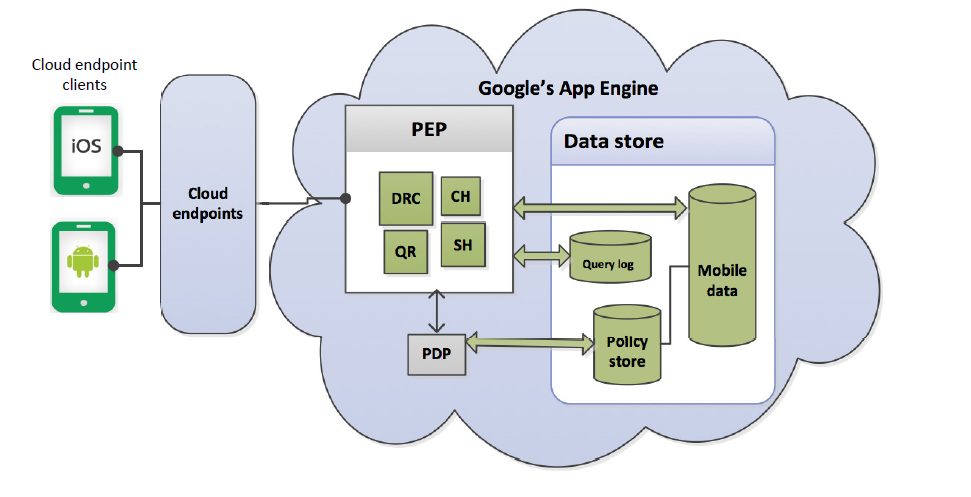
\includegraphics[scale=0.6]{MobiDyc_Private_Mobile-Based_Health_Data_Sharing_Through_fig1}
	\caption{Zarządzanie dynamiczną polityką prywatności. Obraz pochodzi z pracy \cite{Ammar2014}}
\end{figure}


\subsection{System HealthNet \cite{5534981}}
HealthNet jest systemem do mobilnego, elektronicznego monitorowania zdrowia i zbierania danych. Składa się z sieci sensorów ("body sensor network") osadzonych w ubraniu. Czujniki komunikują się bezprzewodowo z telefonem komórkowym użytkownika, który odpowiada za zarządzanie, trzymanie i transferowanie danych w sposób bezpieczny. Dane mogą zostać przetransferowane do ekspertów medycznych, opieki w nagłych przypadkach i prywatnych osób, którym ufa użytkownik. To użytkownik kontroluje kto ma dostęp do danych. Tylko lekarze medycyny ratunkowej, znajdujący się w pobliżu pacjenta mogą uzyskać dostęp do jego ważnych danych bez zgody indywidualnej użytkownika. Praca opisuje unikalne funkcje, związane z bezpieczeństwem i prywatnością. 

\begin{figure}[h!]
	\centering
		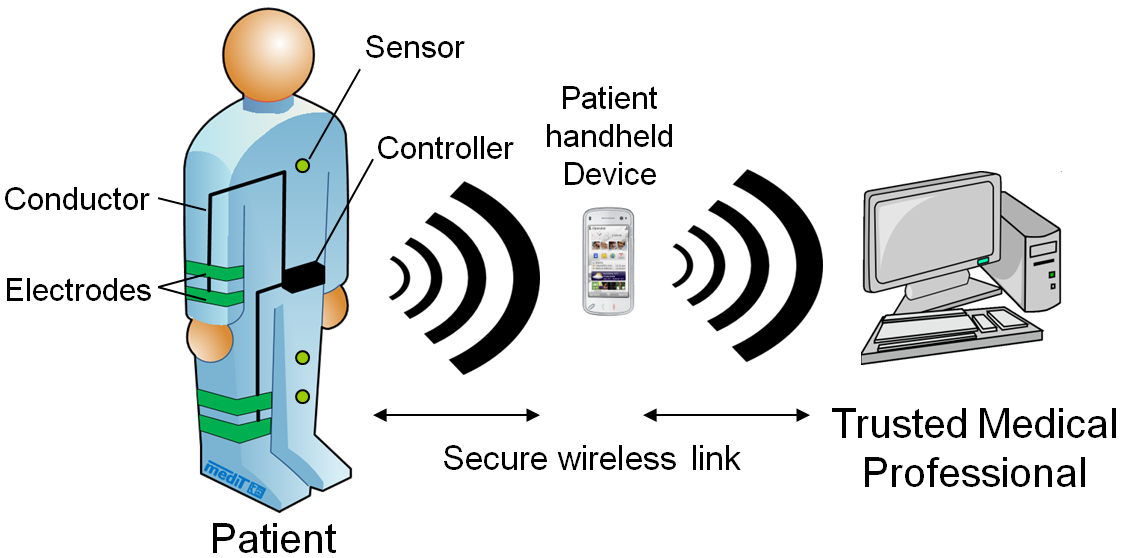
\includegraphics[scale=0.3]{Security_and_Privacy_for_Mobile_Electronic_Health_Monitoring_and_Recording_Systems_fig1}
	\caption{Opis scenariusza HealthNet. Obraz pochodzi z pracy \cite{5534981}}
\end{figure}
